\chapter{Model MAIN VERSION IN OVERLEAF UNTIL MOVED BACK} 
\label{Sec:Model}

%We build a spatially explicit agent model where agents work in one location and have transportation costs to travel to work. 


This work integrates a model of production and labour into a standard spatial model of the city. 
In this chapter, we introduce an analytic model of production and a labour market in a stylized circular city. 
We develop a spatial model with a labour market and agglomeration effects consistent with the literature as our base model. 
% Extended appropriately, this basic model could be used for planning.
We take a step beyond integrating labour markets in a city, to studying the distributional effects: who gets the surplus, what does that mean for the class structure, and ultimately the productivity of cities? 
% In this section we introduce the production function, introduce the labour supply and the urban model, the source of the surplus, then we calculate profit, consider who gets the profit, and from there we draw our conclusions.. then we calculate the urban surplus, and consider who gets it. 
%In subsequent sections we relax assumptions and look at how the interaction between the production of social wealth in cities interacts with housing and the extraction of rent to drive patterns in a richer model with heterogenous agents interacting over space and time. 
In the next chapter we will integrate a version of this production model in a spatially explicit agent based model with financialized investment. 

This model has two parts, first a production function, modelling how urban regions generate wealth, and second a model of an urban housing market. 
In this section, we introduce the basic structure of the model and examine the effect of agglomeration, using a circular city model.  
The model has a Solow-Swan style production model with agglomeration effects.  
It incorporates Jacobs-style labour-augmenting agglomeration economies 
%(Beaudry and Schiauerova 2009, Panne 2004, J. Jacobs 1969), 
in the way the Solo-Swan model incorporates labour-augmenting technical change, using a Cobb-Douglas production function. 
It then integrates the production function with an Alonso-style urban model of a city economy (Alonso 1964). 
It is a model of a productive economy since the centre is productive and demands labour.

% Alternative phrasing 
%We integrate a labour market into a spatial urban model, set up to explore rent, and implications for the distribution of wealth.
%This model has two parts, first a production function, modelling how urban regions generate wealth, and second a model of an urban housing market. In this section introduce the labour supply and the urban model, we model the production function, then we calculate profit, consider who gets the profit, and draw conclusions. % The work draws on the Alfonso/Von Thünen model of the concentric city and Dawn Parker and Filatova's work in agent based modelling of housing markets (see http://jasss.soc.surrey.ac.uk/12/1/3.html 2009).% We begin with a simple model of a circular city with urban agglomeration effects. In subsequent sections we will use an agent based model to relax assumptions to look at how the interaction between the production of social wealth in cities interacts with housing and the extraction of rent to drive patterns for individuals over space and time.

The result is a simple model in which marginal productivity determines the wage, the wage determines the size of the city, the size of the city determines the labour supply, and labour supply determines marginal productivity. 
The model is constructed so that there is neither land rent nor capitalist exploitation in the rural economy. 
This special case allows us to examine the distribution of the social surplus generated by agglomeration economies and the effect of financialization.

In the simplest model, the central place pays a uniform wage, $w$ to all employees, who have identical preferences and transportation costs. $w$ is an attribute of individual residents. Residents  purchase or rent equal quantities of land at differing locations $l$ for identical housing.  

There are transportation costs $T$ that depend on distance from the  central place, so land close to the central place is more attractive than land farther from the central place.  

The equilibrium concept is that a market with identical individuals with identical incomes and transportation costs will result in identical utilities. The result is that land rent must decline with distance from the central place to offset rising transportation cost. 

The size of the city is determined by population and lot size. Income and transportation costs will interact with lot size. The basic model can be initialized by matching the number of properties to the size of the population. 


\subsection{A Circular City}

%Call it a radial city?
Following the Alonzo model [], firms are located at the centre of a circular city, the central business district. Residents residents live, spread across the space, and can take jobs and commute to work.
%In the simplest version, firms concentrate at the city centre. Workers are spread over space and pay transportation costs to commute.

Firms produce goods to sell. They can produce more goods by hiring additional workers. 
There is an agglomeration effect, which means firms can also produce more goods by operating in a city with more people, because of the connections and interactions between people (CITE). 
The simple circular city can be extended to to produce other forms, including polycentric cities and hierarchies of cities at the cost of additional computational complexity. The simple case we examine will allows us to focus on the general, and neglected, distributional features of this class of models.

\subsection{Labour Supply}

%The wage  determines how far people can travel, since it pays for subsistence, that surplus can go to travel, so the higher the wage, the farther workers travel for work. \note{Maybe } 

Workers in the countryside receive a subsistence wage, $\psi$, which could come from work in the local community, living off the land, family support, social support, or something else. % cite other models with subsistence wage.

Firms pay a wage premium, $w$, over the subsistence wage to attract workers. 
When workers take a job, they give up the subsistence income and instead receive the wage from their employer. 
The total wage employers pay is thus the subsistence wage plus the urban wage premium  $\psi + w$.
Specifying the model in terms of a wage premium simplifies the link to the production side and the treatment of household choice.

The urban wage premium determines how far people can travel. The higher the wage, the farther workers travel for work. 
Workers will go to work if the wage premium is greater than the cost of travel, $\tau$ per unit distance. 
Wage and transportation cost therefor determine the radius of the circular city, which determines the size of the labour force which affects urban productivity.  The cost of travel is therefore an important variable in the development of urban productivity. 

%Living close to work has value to workers because it saves the cost of transportation. 
%We assume workers receive a subsistence wage, $\psi$, in the countryside, which could come from work in the local community, living off the land, family support, social support, or something else. % [MAYBE ADD This follows xyz's approach, and makes it possible to explore resident's choice to work]. 

%If the cost of transportation is $\tau$ per unit distance, then t
The farthest workers will travel to work is thus $\frac{w}{\tau}$, which defines the radius of the commuter shed. Thus a worker, located at a distance $d$ from work, paying as much as $w-\tau d$ in rent, would still choose to work, and the maximum distance that workers will commute is the radius of the commuter shed. Given a uniform lot size $s$, with one worker per unit land, the labour available is the area of the city. In the circular city, this is the area of the circle divided by the lot size
\begin{equation}
                 L%=  \frac{\pi}{s}(c^{max})^2	
			=\frac{\pi}{s}  \left(\frac{w}{\tau}\right)^2
			=\frac{\pi}{\tau^2 s} w^2, \label{Eqn:LabourSupply}
\end{equation}
which increases with the square of the wage. This is the equilibrium urban labour supply curve.

As in the standard circular city model the constraint on city size and hence growth is provided by transportation costs, which limit the size of the labour force at any wage. 
% Rising transportation costs can become the limit on firm or city expansion. 

%To get wage, we can write thee  inverse labour supply function  is
%\begin{equation}
%	w= (\frac{ \tau^2s}{\pi})^{0.5} L^{0.5},	%\label{Eqn:InverseLabourSupply}
%\end{equation}

 % TODO:  FOOTNOTE the transportation cost/distance relationship appears to be non-linear in many cases. While the linear model connects with the established literature, we likely want to explore the implications of more empirically grounded curve (e.g. Alain Bertaud, 2015)
% More generally, if we were to introduce variations in lot size and housing types  we would want the integral of the worker density function. In our ABM version  of the model we simply count the workers within the commuter shed.

% DETAILS AND ALTERNATIVE PHRASING  
% MARGINAL PRODUCT The marginal product of labour is monotonically declining, ensuring a labour market equilibrium, to connect with the analytic tradition of economic modelling by ensuring there is an equilibrium level of production.  While adding more labour may always adds some value, the rate at which it adds value drops off. 
% If the marginal product increased, then a firm that got large enough would out compete smaller firms, hire all labour, always be able to produce more wealth by hiring more people, and would always produce more wealth by hiring people than by firing people. This doesn't happen. 
% Perhaps, the firm hires employees who best fit its needs first, but to grow, eventually it must hire less selectively. Finding markets may get harder with growth. Perhaps expansion adds additional costs, building a parking lot, administration, acquiring a larger building. Whatever the explanation, the marginal product of labour declines. 

% Frictional unemployment usually just refers to people moving between jobs. When people look for jobs, it may take time to get them. The analytic model offers an equilibrium solution with full employment. In the agent based model this assumption does not hold, workers are laid off, and take time to find new employment.
% labour adjustment costs include moving costs for the employee or hiring, firing, or training cost for the firm. (there might be a hiring, firing, or training cost on the firm side, or on the employee side: expected time to employment costs, moving costs, etc.)
% The assumption of monotonically embedded marginal product of labour is embedded in the production function, so it applies in the analytic and agent models. This appears in the requirement that the sum of the exponents in the Cobb Douglass are less than one without agglomeration effects. Agglomeration effects can push the sum above one. When the exponents add up to less than one, there are diminishing returns to scale.  Exploring alternatives would involved exploring other formulations of the production function.

% $mvp(x) = p(x)$ where x can be labour, capital or any other factor, falls out of the function when you introduce profit maximization. Continuity and differentiability assumed but it is a convenient approximation-- take away assumptions you typically get a close approximation.

%We have a two factor model of production with labour and capital.  


\subsection{Production}

Firms produce goods which they sell in a commodity market\footnote{For simplicity, assume firms produce a variety of perfectly substitutable commodities which are exported and locally consumed at a fixed price in a large market. Note increasing product variety may produce a consumption agglomeration economies as in \cite{FujitaKrugmanVenables}.}. Demand for the urban product is perfectly elastic which means producing more won't affect the product's price; and there are decreasing returns to scale, which means each new worker increases output by less than the last worker did. 
  
We use a two factor model of production, where production, is a function of capital and labour. The firm maximizes profit by setting the marginal value of the product of each factor equal to the unit cost per factor. We model agglomeration with a Solow-Swan style term for labour augmenting technical change. In the Solow-Swan model 

 \begin{equation} 
Y(t)=K(t)^{\alpha }(A(t)L(t))^{\beta }
\label{Eqn:Solow-Swann}
 \end{equation}
where $Y$, $K$ and $L$ are aggregate output, capital, and labour, respectively,  $A$ is the term the Solow-Swan model introduced for technology, that can capture the growth of labour productivity over time, $\alpha$ is the elasticity of output with respect to capital, $\beta$ the elasticity of output with respect to effective labour, and $t$ time. If $\beta=1-\alpha$, this is a constant returns to scale (CRS) production function at the firm level.

% In the Solow-Swan model all factors of production are fully employed, and initial values $A ( 0 )$, $K(0)$, and $n( 0 )$  are given. The number of workers, i.e. labor, as well as the  level of technology grows exogenously at rate %s are $n$ and it   $g$,% respectively:     $L(t)=L(0)e^{nt}$     $A(t)=A(0)e^{gn}$ 
 
This model uses a similar functional form to look at  the effect of population density increasing % productivity. %how density increases in in  % It models how population increases productivity. $\Lambda(n)n$ is  ``effective labor'' 
 the productivity of labour, rather than technology growing productivity over time. With labour augmenting agglomeration, $\Lambda(n)$, in place of technology, the equation becomes 

\begin{equation} 
Y=K_i^{\alpha }(\Lambda(n)n_i)^{\beta }.
\label{Eqn:Prod1}
\end{equation} 
where $n_i$ is the number of workers at the firm, the labour, and $n$ is the urban population. The agglomeration factor increases with population. It multiplies labour because agglomeration scales the productivity of workers. 

A natural functional form of the agglomeration effect for illustrative purposes n is $\Lambda(n) = n^\gamma$. Then:

\begin{eqnarray}
 Y&=K^{\alpha }(n^{\gamma}n)^{\beta}  \nonumber\\
 Y&=K^{\alpha }n^{\beta(1 + \gamma)}.
 \label{Eqn:Prod2}
\end{eqnarray}
If $\gamma=0$ there are not agglomeration effects. Notice that  this formulation implies it is possible to have increasing returns to scale for the urban economy even with a production function at the firm level with decreasing returns to scale: the return to the total economy $\alpha + \beta(1 + \gamma)$ can be greater than one, even if $\alpha +\beta$ is less than one. %.\label{Fn:PSI}}  
(CITE Appendix: Excess Returns)

Assume $\Lambda(1)=1$ so the agglomeration effect has no influence with one person in a multiplicative function like the Cobb-Douglas, and $\die{\Lambda}{n}>0$, so it is increasing with population.

%%%%%%%%%. ***WHY
If $\beta=1-\alpha$, this is a constant returns to scale (CRS) production function. Without agglomeration effects, $T(n)=1$,  Then  \textbf{$\mathbf{L(n) = T(n) n}$} 

% Without agglomeration effects, $\Lambda(n)=1$,  Then  \textbf{$\mathbf{L(n) = T(n) n}$} }

% Firms will purchase the time of workers to capture the product of their effective labour % and enjoy the product of effective labour. %was If labour markets are competitive, it will set 
%$\die{Y}{L}=w$.
%*** DEFINE EFFECTIVE LABOUR, COMPETITIVE MARKET
% Effective labour is the productive output from labour. As soon as you introduce agglomeration economies, labour becomes a more complex phenomena. There is the benefit of the single worker which should be perfectly declining on that nice concave production function and there is the diagonal movement as a result of increasing productivity because you keep adding people to the market. That means that your productivity of the worker isn't' just attached to the worker and your plant. It has this other component.. 'effective labour' -- the output including the A term.
% Labour always depends on the human capacity, technology, tasks aside so it is always complicated
%Capital is always complicated too it has dates, whether you can get the inputs for it, whether they're produced nearby etc.. -- 

%** ``The notion that your labour force is on average more productive when there are more people around is pretty dramatic and it's very much not part of the basic model that we use. Our starting point is that's the fundamental feature of cities, and what does that do with financial capital and what does that do to distribution and that's not been explored.

%Competitive market- everybody is a price taker they don't assume.
%price takers don't assume anything you do affects other producers or suppliers .. so you act in terms of account your internal prices and costs.
%Take into account any one else's behaviour
%the easy way to see that is assume prices are fixed - all that's required to get the behaviour.

%* have a few other things like free exit and entry, perfect information etc -- to get the efficiency result. - (or to ensure price taking)

%Monopolists knows that increasing output will require a reduction in price-- and take into account how consumers will apply and take it into account.
%No externalities imperfect information etc.. ensure efficiency but aren't needed, all you need is price taking for individuals to only pay attention to their own costs and their own benefits. 

%competitive markets many sellers, many buyers, monopoly single seller, monopsony - single buyer, intermediate cases - monopolistic competition - with some market power but not complete - duopoly- some inefficiency depending on the behavioural model because in the duopoly case they may be able to take advantage of the behaviour of buyers.
% Start with perfect competition, then introduce monopolistic competition is most likely.. but it's more difficult to handle. e.g. with brand names, people have some preference for some feature of your particular good so you can price it higher even though you may loose some marginal people. Firms compete on brand name and reputation, not the pure cost effect.
% In the spatial economy, goods are deferentially interchangeable. Put them on a line and firms pick a place along they line. Firms are in competition but are competing on a line-.. spatial model moved over to characteristic space.. -- looking at this would involve overlaying another space - the characteristic space on the physical space. .. There are also local places with local grocery stores. Polycentric stores have effectively monopolistic competition in real space. - like a named cafe downtown has the same.
% Market power means you can price above marginal costs. Need free entry to get rid of it. -- it doesn't drive out profit - profits can be sustained over longer.
% Monopolist can charge a higher price but pays competitive price for all inputs including labour. If a firm also had a monopoly on offering jobs, they could drive down wages.

%Firms calculate what the next worker is worth to them. That's what they're willing to pay for labour. 
%This is the labour demand function based on the marginal product which is declining. When a firm has only a few workers, it is high on that demand function, and has to move down. It cuts workers. If it's too low, it expands and hires. Note this says something about the geometry of what employers could pay. Firms can't pay workers more than they can earn in the long term, unless that money comes from somewhere, but they could push down wages and extract more profit, invest more in other factors of production, etc

To maximize profit 
% firms set the marginal value product of labour, $p\die{Y_i}{n_i}$, equal to the wage. 
in a competitive market, firms offer a wage equal to marginal value of labour, $p\die{Y_i}{n_i}$, where $i$ indicates the $i^{th}$ firm. In the analytic model, there is no frictional unemployment, there are no labour adjustment costs.\footnote{Note: we do not assume equilibrium conditions in the agent model, however our approach is to stay close to the analytic tradition, relaxing assumptions to clarify what drives each results, and connect the work with classical and neo-classical theory.}. % For instance in the agent model, employees are simply laid off and seek work, so there is unemployment, but there are not labour adjustment costs for firms.}. For convenience, price per unit is one. 

A labour market equilibrium exists if the marginal product of labour, is monotonically declining, which it is with a Cobb Douglas production function, and $\alpha + \beta<1$ 
Population would be expected to adjust much more slowly than firm wages, so labour supply should converge. The case where there are increasing returns at the city level introduces interesting dynamics, explored in appendix CITE % 'furthur discussion' appendix.

%To ensure there is a labour market equilibrium to study in the analytic model, the marginal product of labour declines monotonically, 
%***ILLUSTRATE AND CLARIFY
%If you see it as just supply and demand .. 
%Supply demand with fixed product and everything’s neat
%Agglomeration changes everything,.. firms are underestimating each time they add a worker, the value that’s going to be produced. They benefit from an agglomeration effect and that’s where they interesting dynamics are coming from..
% we know that there is a marginal product of labour for a firm that it should be able to figure it out.. can the person on the shop floor figure out whether it's worth hiring another person.. we can talk about it, add details etc. We have a declining marginal product of labour. Because of transportation costs, we have a rising cost of getting labour so they cross and there is an equilibrium. There are adjustment questions like which adjusts quickly, how fast people move in, how fast firms decide to hire etc, but we know that there is in principle and equilibrium and that it is in principle a stable equilibrium (DIAGRAM STROGATS) although there are complications with this-- some argue these market equilibria never make sense- true in lots of way, but useful for analysis. 
% The question is then, what happens in our city? Do you get a growth dynamic? What seems to be the case is that if all the firms add workers then the marginal value of the product of all the workers they have goes up, which means they are making more profit which means if they are making more profit they want to hire more workers? Does it ever converge? Likely eventually, but it's got a very powerful dynamic.  If you add other features like more products being created in the city, which is part of this agglomeration process you can start seeing, if you exhaust one source of growth, we know that there are others, that simplification is just firms of the same sort hiring workers of the same sort is wrong. so we need to add the local service sector, we need to add the possibility of creating new products and those depends on the number of workers and so depend on further agglomeration effects. What does this mean? For the purpose of the model, we'd want to strengthen the agglomeration effect relative to what they are for specific firms or industries..

Population/workforce, $n$, and the wage will be determined endogenously in competitive markets. 


\subsection{Rent}
\label{Sec:Rent}

%``We model how land rent is captured by landowners and how that affects wealth creation and the development of the city. 

%Land is a monopoly good \note{talk about what you mean by monopoly good?} 
The supply of land at any distance from the center is inelastic. 
Its value comes from proximity to the productive urban centre, not from the value of improvements made to the property. 
% Reference sections on development which is different, and the contribution of amenity % Because supply is fixed for urban land, and the landowner has a monopoly claim on rents, the rents that can be depend on wages and amenity rather than the cost of improvements made to the property.
% The source of rents is the free gifts of nature, the coming together of people to create value in cities, and the concentration of public amenity in cities. 
In the circular city with linear transportation costs, the maximum rent for living closer to work is at distance $r$, from the center, is $w-\tau r$.  is Workers could pay that much and it would still be worthwhile to commute to work. 

Rents go to landowners. %the owners of a given property. 
Landowners therefore capture a fraction of the wage premium generated by agglomeration.

If workers own their own homes, rents go to them. If others own the land, they capture them. %\note{REPHRASE? rent is  extracted from the coalition of capital and workers.} % Rents may also be taxed, could be shared between multiple owners, etc. 
%The rents are captured by landowners.  The capture of rents by landowners is common buy not necessary. 
In principle the gains from urban productivity and amenity can be allocated as social wealth through shared ownership, as is often done on a small scale with cooperatives and land trusts, distributed to all citizens through something like a social wealth fund, or captured in taxes or fees as Henry George suggested. 
%The rents would otherwise go to labour and capital.

% Agglomeration benefits get extracted by landowners. Labour gets only their marginal value they don't get any of the surplus. They don't even keep always their marginal value.
the dynamic story is that the class of landowners eventually becomes financial capital.
PLOT RENTS HERE

The value of land increases over time. Those who purchase land earlier claim a share of the growing value of the city. % As the city grows, they own an increasingly valuable asset.
 
%In this model, workers are the initial owners, but they build this wealth which becomes a source of capital that can support them.

EQUATION FOR THE SHARE THEY CAN CAPTURE


\subsection{Demographics}

Workers can leave the workforce and retire, and new people can come into the city. Land value rise as the city grows, so newcomers pay more for housing near the centre.

In the case in which individual workers purchase houses and then sell them on retirement, the housing market drives the creation of classes on its own. A strictly random process in which agents have a range of ages and sell at retirement creates a structural advantage where workers who arrive earlier in the city and own land, benefit from their own labour but also get to claim a share fo the productive output of the city as it grows. % those who begin work later. % to a division in wealth
%the emergence of a class of those who came early and those who came late.
%Early agents may also rent out their land. Could it be though of as a pyramid scheme?

In the classical language, someone is exploited if someone else gets a share of the value of their labour. %(REPLACE WITH MORE PRECISE DESCRIPTION). 
 Employers capture a share of the value of workers' labour, so they exploit workers under this definition.
Those who own land early in a growing city are also capture a share of everybody's production. Since they capture a share of the productivity of others working in the city, through the rents, they are also exploiters, they form a kind of hybrid class. %Rents could be captured directly through renting out the property after they retire away from the city,  or by selling the property at a higher value than they bought it. 

% MARGINALIST DISTRIBUTION
%we've been paying some people less than the market wage so our profits our higher. this is what it would be if we paid everybody
% FOOTNOTE - RELATIONSHIP with marginalist distribution story ******** TODO Does the marginalist approach assume they are not exploited? Is it an experiment in examining the case where production is non-exploitative? 
% In a sense if labour gets the marginal value of their product, are they exploited. It's a matter of interpretation.  -It has an attraction 
%Clark tried to make an ethic of this. if everyone is being paid the marginal product of their labour. We know that's an efficient outcome. If it's efficient, is it also fair
%Is it possible someone's taking out an extra large fair. Yes. Not fair for simple classical reason that labour has been exploited in the past and that the current owner ship is a result of exploitation. The ownership of land introduces a kind of exploitation-- clearly exploitation if you claim that. 
%Lot's of marxists didn't like Henry George making it a locational question, they wanted to keep it located in the factory.
% You could - well what value did they create -- in line with those other-- could interpret.. 
%What is the average value, because every worker is not just marginal, they're also average/identical. What is the value created by the whole of the workforce. Should they be paid the marginal value or the average value of their work.
%
%The avg value -- declining.. 
%The demand for labour is declining--  
%Every infra marginal worker has been paid less than the avg contribution 
%Every infra marginal workers should - 
%every marginal worker should get the average wage.. that's fair.
%
%Get to the margin - that's what you pay.. that's what the next worker is worth to the firm. .. 5th' worker is paid more than the 10th. should it be averaged out and paid to all workers? paid to worker, or should the difference between top and the marginal goes to the firm- -- that's profit.. pay everyone the marginal value and keep the rest as profit.. 
%Effective labour has a higher marginal product.. - even higher - higher for the firm.. - but they don't have to pay the workers that... firms only have to pay enough to get their marginal individual cost down to the wage. The problem there is if they're making more profit they want to expand the workforce, but that wage only supports a certain size of city -- they've got off raise the wage a bit.. so they face an upward sloping supply curve for labour=-- that's why you know there's an equilibrium.. declining product and upward sloping supply so they cross.
%
%(all the profit you earn on the way could be redistributed)

\chapter{Land Market}

Urban productivity %and amenity
drives land values through the housing market.%Agents purchase homes to live in. The value of the the proximity to work and to amenity drives shapes the what agents are willing to pay. 
% These prices shape the relationship between housing markets and the wealth of households.
Our goal is to look at the relationship between housing markets, financialized investment, and production. % and labour markets. 
To explore this relationship, we integrate the model of production developed above with a spatially explicit agent based land market. % in which heterogenous individuals and institutions buy and sell properties given their individual goals, resources and available information. We integrate this housing market with % within this model of individual and institutional actors in a spatially explicit property market, a model of production and employment.

We examine the effect of housing on wealth inequality by looking at 
%We explore the wealth forming dynamics of the urban agglomeration effect by modelling 
a city in which agents work in the city and leave their jobs when they reach retirement age. They may choose to rent or sell their home. %?They may chose whether to stay in the city, if there is sufficient amenity value for them, to rent their house, or to sell it. % Todo can agents choose not to retire? Can they keep working? Do they get the subsistence wage on retirement? Do they need to leave the city to get it? 
New agents enter the city to work. 
Agents fund their retirement from savings, as well as returns on their home if they own one. Savings may be invested in a pension fund, or in local property,  depending on expected risks and returns. % either in the stock market, or in pensions.
A financial institution manages the pension, investing in the market or in property.
%Institutional and individual investors can access debt. %We also consider a case where outside money can come under institutional management, not just local retirement savings. A parameter controls the inflow of additional money beyond local investment in the pension fund. 

% There is an outside world in two respects. There is a market for the urban product produced by firms, and a financial market that agents can invest in.
% Lots of simple extensions e.g. 2 cities with immigration, differentiated labour, products, market power, neighbourhood effects (see extensions map/typology), we focus on those elements central to seeing the structure of the resilience dynamics of the wealth/housing effect. Consider adding density, to look at how it interacts with agglomeration effects. (integrating with transportation effects is very neat)
 
 If there is a housing market, agents can move. %In the analytic case above, the population stays in place, and travels to work if it is worthwhile given the transportation costs. 
%Those who come to the city will be those for whom the benefits the city offers make it worthwhile to  whether that's building their network, accessing markets, accessing amenity, learning, finding specialized employment, or increased wages. In this model 
The demand for labour drives urban growth. % The housing market depends on how many people from the periphery are completing to claim places in the city. TODO IF ANY RURAL AGENT COULD MOVE IF THE CITY HAS ADDITIONAL DEMAND FOR LABOUR, HOW DO WE DECIDE WHICH DO? Could use a parameter for immigration (or how 'hot' the market is) and in the simplest case (corresponding to how many agents from outside are looking at the housing/rental market), have the inflow match. % Agents have debt and there is an undifferentiated labour market
 % We may. 
 
Figure xyz traces the flow. In each time step agents firms update wages and job availability, agents decide whether to work and whether to buy and sell homes.
 % Schedule: Multi step by breed
 % Steps Labour
 % step - workers: market/production, enter market to buy, list properties real estate agent matches agents - has bids 
 % bidding - workers and firm consider properties and make bids (2nd step or spread over 2 steps)
 % negotiation - sellers consider and accept bids (or real estate agents manage negotiation)
%Buyers evaluate their need for housing.
% Agents decide whether to enter the housing market as a renter or a buyer.


 
Worker agents from outside the city can always consider moving and accepting a job. % QUESTION - how to manage the flow of new agents?
%, or can make more from rents and moving away (with a non-differentiated workforce)
% They need to approximate housing prices to know if it makes sense to work. Do they use past prices?
% 
% 
The higher their need, the more houses an agent considers, and the more willing they are to negotiate on price. % Buyers rank their housing need on a scale of one to ten. 
% Maybe later: Buyers could consider neighbourhood pressures, demographic changes, changes in job location, desire for amenity etc. in their assessment of housing need. 
Buyers then consult with a financial agent to determine the maximum mortgage and interest rate they'd qualify for based on their income. This gives an upper bound to the range of homes they may consider. 

Next buyers request a selection of homes to consider from a real estate agent. Those with higher need for housing look at more homes. The real estate agent offers a selection of homes based on the agent's requirements. A randomness parameter determines how many divergent houses are also considered. When the parameter is 1, the selection of homes is fully randomized, When it is 0, the agent sorts all available homes and offers those which fit the agents budget, space, and other requirements best.

Finally agents rank all the homes offered and place bids.  For simplicity of implementation, they place bids on all homes they consider. They place the most competitive bids on those homes they prefer. If they have higher urgency they place strong bids on more homes. 
A utility function/algorithm specifies agents preferences over the attributes that matter. - algorithmic continuous. lexographic- any traits. 

Finally Variables from last time also affect desire and urgency in the next time step. If there is a good fit/price ratio, their assessment of desire increases. If they dislike what they see, their desire decreases -- they settle for what is there. 



%Calculate willingness to pay
%Consider options
%Place bids
%
%Calculate willingness to pay (urgency/position on the market)
%Assess need for housing
%- Urgency of need Unhoused, sold house or served notice? 
%- Family or demographic changes
%- Financial viability of current situation
%Assess financial situation
%Get Max mortgage and max carrying cost given income and wealth from a bank
%Get options from real estate agent
%Place bids based on xy
%Consider options
%Place bids
%
%
%
%BUYER
%
%Enter market to buy
%Decide level of urgency (or decide with prospect theory - functional form for optimism/urgency/time to choose)
%(income/wealth)
%Maximum mortgage 
%Maximum carrying cost
%Household attributes - household size, employment location, amenity
%Current housing
%
%Realtor gives list of houses to look (real estate search -e.g. price range)
%Place offers - low if can't afford, higher if market is tight
%If failed, consider renting or buying next time.


 \tikzstyle{decision} = [diamond, draw, fill=blue!20, 
     text width=4.5em, text badly centered, node distance=3cm, inner sep=0pt]
 \tikzstyle{block} = [rectangle, draw, fill=blue!20, 
     text width=5em, text centered, rounded corners, minimum height=4em]
 \tikzstyle{line} = [draw, -latex']
 \tikzstyle{cloud} = [draw, ellipse,fill=red!20, node distance=3cm,
     minimum height=2em]
%
 \begin{center}
 \begin{tikzpicture}[node distance = 2cm, auto]
     % Place nodes
     \node [block] (need) {Assess need for housing};
     \node [block, below of=need] (finance) {Assess financial situation};
     \node [block, below of=finance] (alternatives) {Select homes to consider};    
     \node [block, below of=alternatives] (bid) {Place bids on homes};    
     % Draw edges
     \path [line] (need) -- (finance);
     \path [line] (finance) -- (alternatives);
     \path [line] (alternatives) -- (bid);        
 \end{tikzpicture}   
 \end{center}




\subsubsection{Financialized Capital}

%Individuals and institutions play a role in the housing market through credit markets and direct investment.Agent's access credit shapes worker's ability to purchase homes. Credit is offered by institutions.
% Agents may be able to foresee future growth. %They may even over invest if they follow market trends and bubbles form. 
% They can claim a share of the urban wealth as it grows over time by owning the land. 

If the return on housing investments is competitive with alternative investments, capital from institutions and individuals will flow into housing. Institutional investors can purchase housing.  Individual households can also allocate a larger share to housing to capture the returns.
% If the return on investment in housing is competitive with alternative investments, can purchase housing for it's financial return. They can rent housing and sell the asset with appreciation later. We examine the conditions in which this increased demand can drive up prices in the market. 
% Capturing future growth of the city, depending on their foresight - how much does it take to block individuals from gains-- Regime.
% both institutional investors and individual agents can purchase additional housing for it it's return on investment even though they don't need it as a place to live. 
% Use value vs rent value. 
%Institutional investors can purchase housing as an investment. Individuals with more wealth may invest 
Households may, for example purchase a larger house than they need, purchasing additional units to rent out, or keep a house after retiring rather than downsizing.  % and individuals with sufficient means can purchase larger homes than they need to benefit from appreciation, or purchase additional units to rent to others. 
% Investors can also purchase housing to claim a share of the future productivity of the city. Individuals and groups can put extra money into housing. Institutional housing providers can buy up the housing supply.
% HYPOTHESIS FEEDBACK LOOP -- FINANCIALIZED INVESTMENT --
%The rise in spending on housing as a proportion of income can be driven by both rising prices (cutting into quality of life) and increasing investment to claim a share of the returns.  -- disaggregate and show the geometry -
% Test how linear is this relationship? 

%With financialization, in the case where 
If financialized buyers can access a better interest rate, they can consolidate ownership, capture rents, drive class differentials, and amplify wealth inequality. % This appears to be the case as lenders offer wealthier and larger entities lower interest rates. % We expect to observe in this class of models larger, likely power law-distributed, wealth effects.

%There is a supply of money- if there's too much for other investments, some will flow here- e.g. excess liquidity.



\subsubsection{Size of mortgage available, $m_i$}
\[m_i= \frac{0.25Y_i}{r_i}\]
where $r_i$ is $i$'s cost of capital, $Y_i$ is $i$'s income.

\subsubsection{Cost of capital $r_i$}
The cost of capital is known to differ for rich and poor. Say for example, the cost of borrowing, $r_i$ for agent $i$ if the base lending rate is $\bar{r}$
 \[ r_i = (A + B \frac{\bar{W}}{W_i})\bar r\]
where $\bar{W}$ is mean wealth and $W_i$ is individual wealth. %Figure~\ref{Fig:BorrowingCost} illustrates the effect.

%\begin{figure}[htb]
%\begin{center}
%\chapter{SAPriceOfCapital}

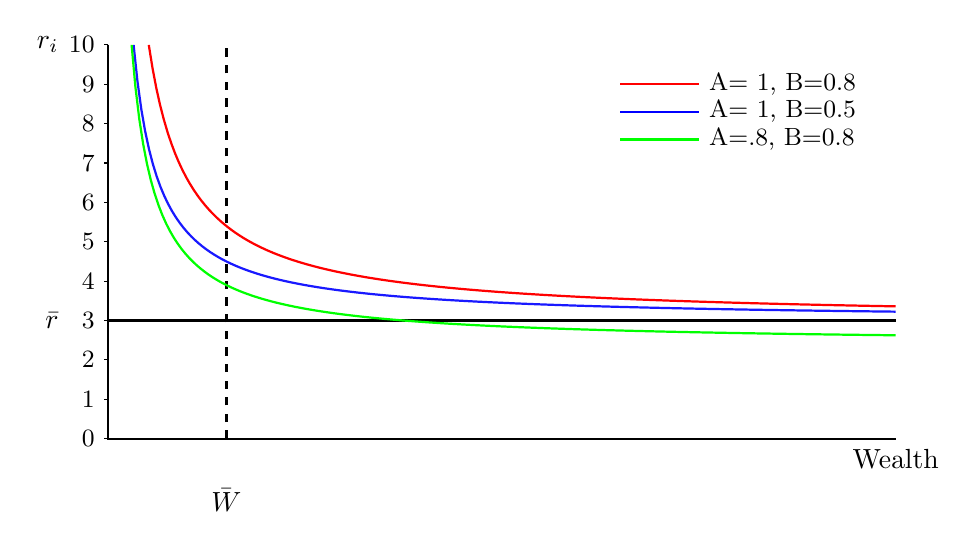
\begin{tikzpicture}[scale=.5]
%\def\bndmax{5}        %https://tex.stackexchange.com/questions/68462/filling-a-complex-region-with-tikz
%\def\bndmin{0.2}
\def \Y {10}  % height of y axis pecent
\def \W {20}  % length  of x axis
\def \Wbar {3} % jmeam wealth
\def \omega {3}
\def \A {1}  %was .5
\def \B {.5}
%Equation   \[ r_i = (A + .5 \frac{\bar{W}}{W_i})\omega\]
\def \Wmin{.63}  %This sets the lower limit fo the 
\def \Wmin{(\B*\Wbar)/(\Y/\omega-\A)} %function to keep in in bounds
	
\tikzset{func/.style={thick,color=blue!90}}	

\draw [thick] (0,\Y)node[left=.5cm]{$r_i$} -- (0,0)--(\W,0)node[below]{Wealth};  	% Axes
\draw [thick] (0,\omega)node[left=.5cm]{$\bar r$} -- (\W,\omega);  	% Axes
\draw [thick,dashed] ( \Wbar,0)node[below=.5cm]{$\bar{W}$} -- (\Wbar,\Y);  	% Axes

\foreach \yi in {0,...,\Y} \draw (0,\yi)--(-.1,\yi)node[left]{\small$\yi$};

\draw[func,domain=\Wmin:\W] plot [samples=200] (\x,{(\A+\B*\Wbar/\x)*\omega});
\def \A {.8}
\draw[func,domain=\Wmin:\W, green] plot [samples=200] (\x,{(\A+\B*\Wbar/\x)*\omega});

\def \A {1}
\def \B {.8}
\draw[func,domain=\Wmin:\W, red] plot [samples=200] (\x,{(\A+\B*\Wbar/\x)*\omega});

\draw [red,  thick](13, 9)--(15,9)node [right, black] {\small A=\ 1,\ B=0.8};
\draw [blue,  thick](13, 8.3)--(15,8.3)node [right, black] {\small A=\ 1,\ B=0.5};
\draw [green, thick](13, 7.6)--(15,7.6)node [right, black] {\small A=.8, B=0.8};
 \end{tikzpicture}
% Figure of cost of borrowing
%\caption{Hypothetical wealth-dependent borrowing cost}
%\label{Fig:BorrowingCost}
%\end{center}
%\end{figure}%

This has a number of immediate implications. First, if agents discount at their borrowing rate, wealthier agents a lower discount rate and therefore value properties more highly. 

Second, given the  common rule that mortgage payments cannot exceed some fraction of disposable income, the wealthy will be able borrow larger amounts and at lower interest rates that the less wealthy. At any distance from the centre they will be able to make a higher bid.
 
If the expected return on a property is greater than the individual cost of borrowing, it would pay any agent to borrow as much as possible and purchase properties as they become available.

\subsubsection{The rate of return on a property purchase $v$}
To explore the implication of the financialization of the urban land market we need a function to calculate the return on a unit of land that reflects the actual gradient of opportunity in financial markets. We begin with the price appreciation, $\Delta P=P_T-P_0 = (1+\dot p)P_0-P_0 $, where $\dot p$ is the rate of price appreciation over the period $T$. Rates will all be specified for the period $T$. Transaction costs, including real estate fees, take a fraction from the value of the final sale.

 The speculator invests a down payment, $D$, and gets back at time $T$ the  increased price $(1+\dot p)P_0$, plus rents, minus any costs and minus the mortgage with interest.
%footnote{We can include a use value, $U$ in place of rent for expatriate owners to represent using the property - say one month a year - when they are not renting the property and a \textbf{vacancy tax},
%$T$ at rate $t$ to affect the speculator's  decision.
 
The rate of return is the value of the gain, $V$,  over the size of the downpayment, $D$, where
\begin{equation}
V =capital\ gain - Interest\ due  	+ Rent  - operating\ cost\    
\end{equation}

The rate of return is $v = \frac{V}{D}$. 

Both the  share of the price  that can be mortgaged, $m$, and the interest rate  and $r$ may be functions of the agent's wealth. $\delta$ represents the net capital gains tax. It makes it possible to capture the capital gains kept. If it is set to one, it simplifies the equations, all is kept. Keeping the variable offers a policy variable to control the return on financial capital.

\begin{eqnarray*}
V  %	&=& capital\ gain - Interest\ due  	+ Rent  - operating\ cost\\
% 	&=& \delta P_T-D \qquad \qquad \quad - (1+\delta r)M \quad	 + R  	-C\\
% 	&=& \delta P _T \qquad-(P_0-M) \quad- (1+\delta r)M 	 + R  	-C\\
%	&=& \delta (1+\dot p)  P_0 -(P_O -M)  -(1+\delta r)mP_0  + R  -C\\
%	&=& \delta (1+\dot p)  P_0 -P_O + M \qquad -(1+\delta r)mP_0  + R -C\\
%	&=&( \delta (1+\dot p)-1)  P_0  + mP_0 \quad -(1+ \delta r)mP_0  + (\rho-\kappa)P_0\\	
%	&=& \left(  \delta (1+\dot p)-1    + m \quad - m(1+\delta r)  + (\rho-\kappa)\right)P_0\\'
%	&=& \left(  \delta (1+\dot p)-1    + m \quad - m-\delta rm  + (\rho-\kappa)\right)P_0\\
&=& \delta(P_T- (1+r)M) \qquad \qquad 	 + R  	-C   - T\\
&=& \delta((1+\dot p)  P_0- (1+r)mP_0)   + \rho P_0  	-\kappa P_0 - tP_0\\
&=&( \delta((1+\dot p)  - (1+r)m) \ + \rho   	-\kappa -t) P_0
\end{eqnarray*}

This is the  net present value of buying, and selling after one period. \textbf{It has  6 exogenous parameters}. Operating revenue and costs $ \rho -\kappa - t$ a present value. 

The rate of return is $v = \frac{V}{D}$. For expat investors, we get a \textbf{decision rule}:\begin{enumerate}
\item  if $v \geq a$ (with some private use?) with no rent,  don't bother renting. 
\item If $v(no\ rent\ and\ tax) < a\leq v(with\ rent)$,  then  rent. 
\item If $ v(with\ rent) \le a $,  then sell 
\end{enumerate}


We can, with some simplifications, write
\begin{eqnarray}
\frac{V}{D}&=&( \delta((1+\dot p)  - (1+r)m) \ + \rho   	-\kappa - t ) \frac{P_0}{D}   \nonumber\\
		&=&( \delta((1+\dot p)  - (1+r)m) \ + \rho   	-\kappa - t ) \frac{P_0}{P_0-mP_0}   \nonumber\\
		&=&\frac{ \delta(1+\dot p  - (1+r)m) \ + \rho   	-\kappa - t } {1-m} \label{Eqn:DecisionRule}
\end{eqnarray}

\subsubsection{Returns on capital are higher for wealthy investors}
\[   r^h=\frac{ \delta(1+\dot p  - (1+r)m) \ + \rho   	-\kappa - t } {1-m}    \]
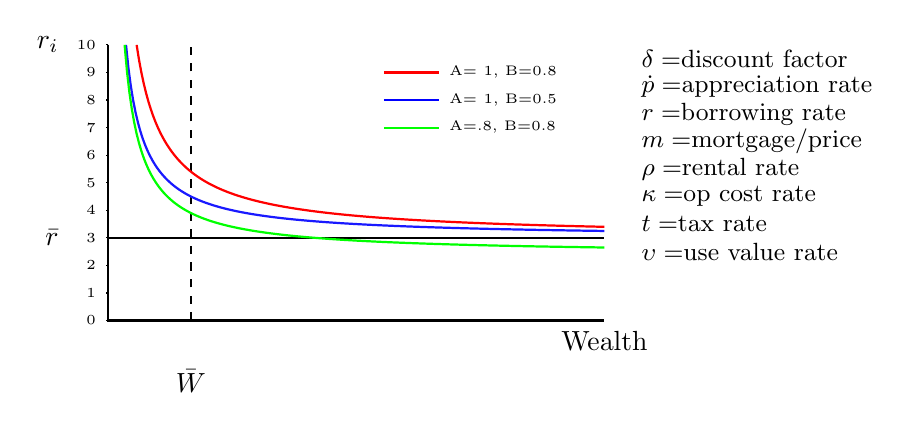
\begin{tikzpicture}[scale=.35]
%\def\bndmax{5}        %https://tex.stackexchange.com/questions/68462/filling-a-complex-region-with-tikz
%\def\bndmin{0.2}
\def \Y {10}  % height of y axis percent
\def \W {18}  % length  of x axis
\def \Wbar {3} % j mean wealth
\def \omega {3}
\def \A {1}  %was .5
\def \B {.5}
%Equation   \[ r_i = (A + .5 \frac{\bar{W}}{W_i})\omega\]
\def \Wmin{.63}  %This sets the lower limit fo the 
\def \Wmin{(\B*\Wbar)/(\Y/\omega-\A)} %function to keep in in bounds
	
\tikzset{func/.style={thick,color=blue!90}}	

\draw [thick] (0,\Y)node[left=.5cm]{$r_i$} -- (0,0)--(\W,0)node[below]{Wealth};  	% Axes
\draw [thick] (0,\omega)node[left=.5cm]{$\bar r$} -- (\W,\omega);  	% Axes
\draw [thick,dashed] ( \Wbar,0)node[below=.5cm]{$\bar{W}$} -- (\Wbar,\Y);  	% Axes

\foreach \yi in {0,...,\Y} \draw (0,\yi)--(-.1,\yi)node[left]{\tiny$\yi$};

\draw[func,domain=\Wmin:\W] plot [samples=200] (\x,{(\A+\B*\Wbar/\x)*\omega});
\def \A {.8}
\draw[func,domain=\Wmin:\W, green] plot [samples=200] (\x,{(\A+\B*\Wbar/\x)*\omega});

\def \A {1}
\def \B {.8}
\draw[func,domain=\Wmin:\W, red] plot [samples=200] (\x,{(\A+\B*\Wbar/\x)*\omega});

\draw [red,  thick](10, 9)--(12,9)node [right, black] {\tiny A=\ 1,\ B=0.8};
\draw [blue,  thick](10, 8)--(12,8)node [right, black] {\tiny A=\ 1,\ B=0.5};
\draw [green, thick](10, 7)--(12,7)node [right, black] {\tiny A=.8, B=0.8};

\def \W {19}  % length  of x axis
\node[right] at (\W,9.5){\small$\delta=$discount factor};
\node[right] at (\W,8.5){\small$\dot p=$appreciation rate};
\node[right] at (\W,7.5){\small$r=$borrowing rate};
\node[right] at (\W,6.5){\small$m=$mortgage/price};
\node[right] at (\W,5.5){\small$\rho=$rental  rate};
\node[right] at (\W,4.5){\small$\kappa=$op cost rate};
\node[right] at (\W,3.5){\small$t=$tax rate};
\node[right] at (\W,2.5){\small$\upsilon=$use value rate};
 \end{tikzpicture}

